\documentclass{article}
\usepackage{pgfplots}
\usetikzlibrary{external}
\tikzexternalize[prefix=tikz/]
% and optionally (as of Pgfplots 1.3):
\pgfplotsset{compat=newest}
\pgfplotsset{plot coordinates/math parser=false}
\newlength\figureheight
\newlength\figurewidth
\begin{document}
\begin{figure}
\centering
%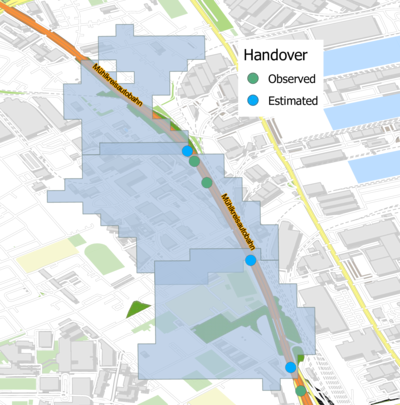
\includegraphics[width=0.7\linewidth]{./images/1058handoveradapted}
\definecolor{mycolor1}{rgb}{0.65098,0.80784,0.89020}%
\definecolor{mycolor2}{rgb}{0.12157,0.47059,0.70588}%
%
\tikzsetnextfilename{1058adaptioncomp}
\begin{tikzpicture}

\begin{axis}[%
width=4in,
height=3in,
area legend,
scale only axis,
xmin=0.5,
xmax=2.5,
xtick={1,2},
xticklabels={{i},{i+1}},
xlabel={Route segment},
ymin=0,
ymax=400,
ylabel={Velocity [km/h]},
legend style={draw=black,fill=white,legend cell align=left}
]
\addplot[ybar,bar width=0.513103448275862in,bar shift=-0.320689655172414in,draw=black,fill=mycolor1] plot table[row sep=crcr] {%
1	396\\
2	80\\
};
\addlegendentry{Without Adaption};

\addplot [color=black,solid,forget plot]
  table[row sep=crcr]{0.5	0\\
2.5	0\\
};
\addplot[ybar,bar width=0.513103448275862in,bar shift=0.320689655172414in,draw=black,fill=mycolor2] plot table[row sep=crcr] {%
1	44\\
2	77\\
};
\addlegendentry{With Adaption};

\end{axis}
\end{tikzpicture}%

\caption{Comparison between the velocity without adaption and with adaption}
\label{fig:1058adaptioncomp}
\end{figure}
\end{document}